\chapter{HASIL DAN PEMBAHASAN}
\label{chap:hasilpembahasan}

% Ubah bagian-bagian berikut dengan isi dari hasil dan pembahasan

Pada bab ini dipaparkan hasil dan analisa dari pelaksanaan tiap tahapan pada metodologi, serta dipaparkan mengenai skenario pengujian dan evaluasi pengujiannya. Secara umum, pada tahapan skenario pengujian terdapat 2 jenis pengujian yaitu: \par

\begin{enumerate}[nolistsep]
  \item Pengujian menggunakan citra tulisan dari penulis berbeda.
  \item Pengujian algoritma konversi gambar menjadi teks menggunakan variasi citra tulisan dari penulis berbeda.
\end{enumerate}

Dengan pemaparan hasil metodologi serta pelaksanaan beberapa skenario pengujian tersebut, dapat ditarik kesimpulan dari pelaksanaan tugas akhir ini.\par

% Skenario pengujian berupa hasil penelitian dan perancangan yang telah dibuat pada bab 3

\section{Hasil Metodologi}
\label{sec:hasilmetodologi}

Hasil dari tahapan yang dilakukan pada tugas akhir ini dijelaskan sesuai dengan metodologi yang telah dibuat. Adapun tahapannya yaitu: \par

\subsection{Hasil Akuisisi Dataset}
\label{subsec:Hasilakuisisidataset}

\noindent Hasil dari akuisisi dataset yaitu didapatkan dataset dengan detil sebagai berikut: \par
% tabel detil preproses dataset
% tabel detil kelas dataset
Secara spesifik, hasil dari tiap proses yang ada pada tahapan akuisisi dataset dijelaskan pada poin berikut.

\subsubsection{Hasil Pengumpulan Citra Tulisan Tangan pada Papan Tulis}
\label{subsubsec:hasilpengumpulancitra}

Proses pengumpulan citra tulisan tangan papan tulis dilakukan dengan menuliskan sejumlah huruf pada media papn tulis kemudian dilakukan proses pengambilan gambar. Proses tersebut diulang selama beberapa kali untuk setiap kelas huruf, dan diulang sejumlah kelas hurufnya. Seluruh tulisan tangan pada papan tulis ditulis oleh 1 orang yang sama. Contoh hasil pengambilan citra dapat dilihat pada gambar \ref{fig:contohcitratulisantangan} berikut. \par

\begin{figure}[H]
  \centering
  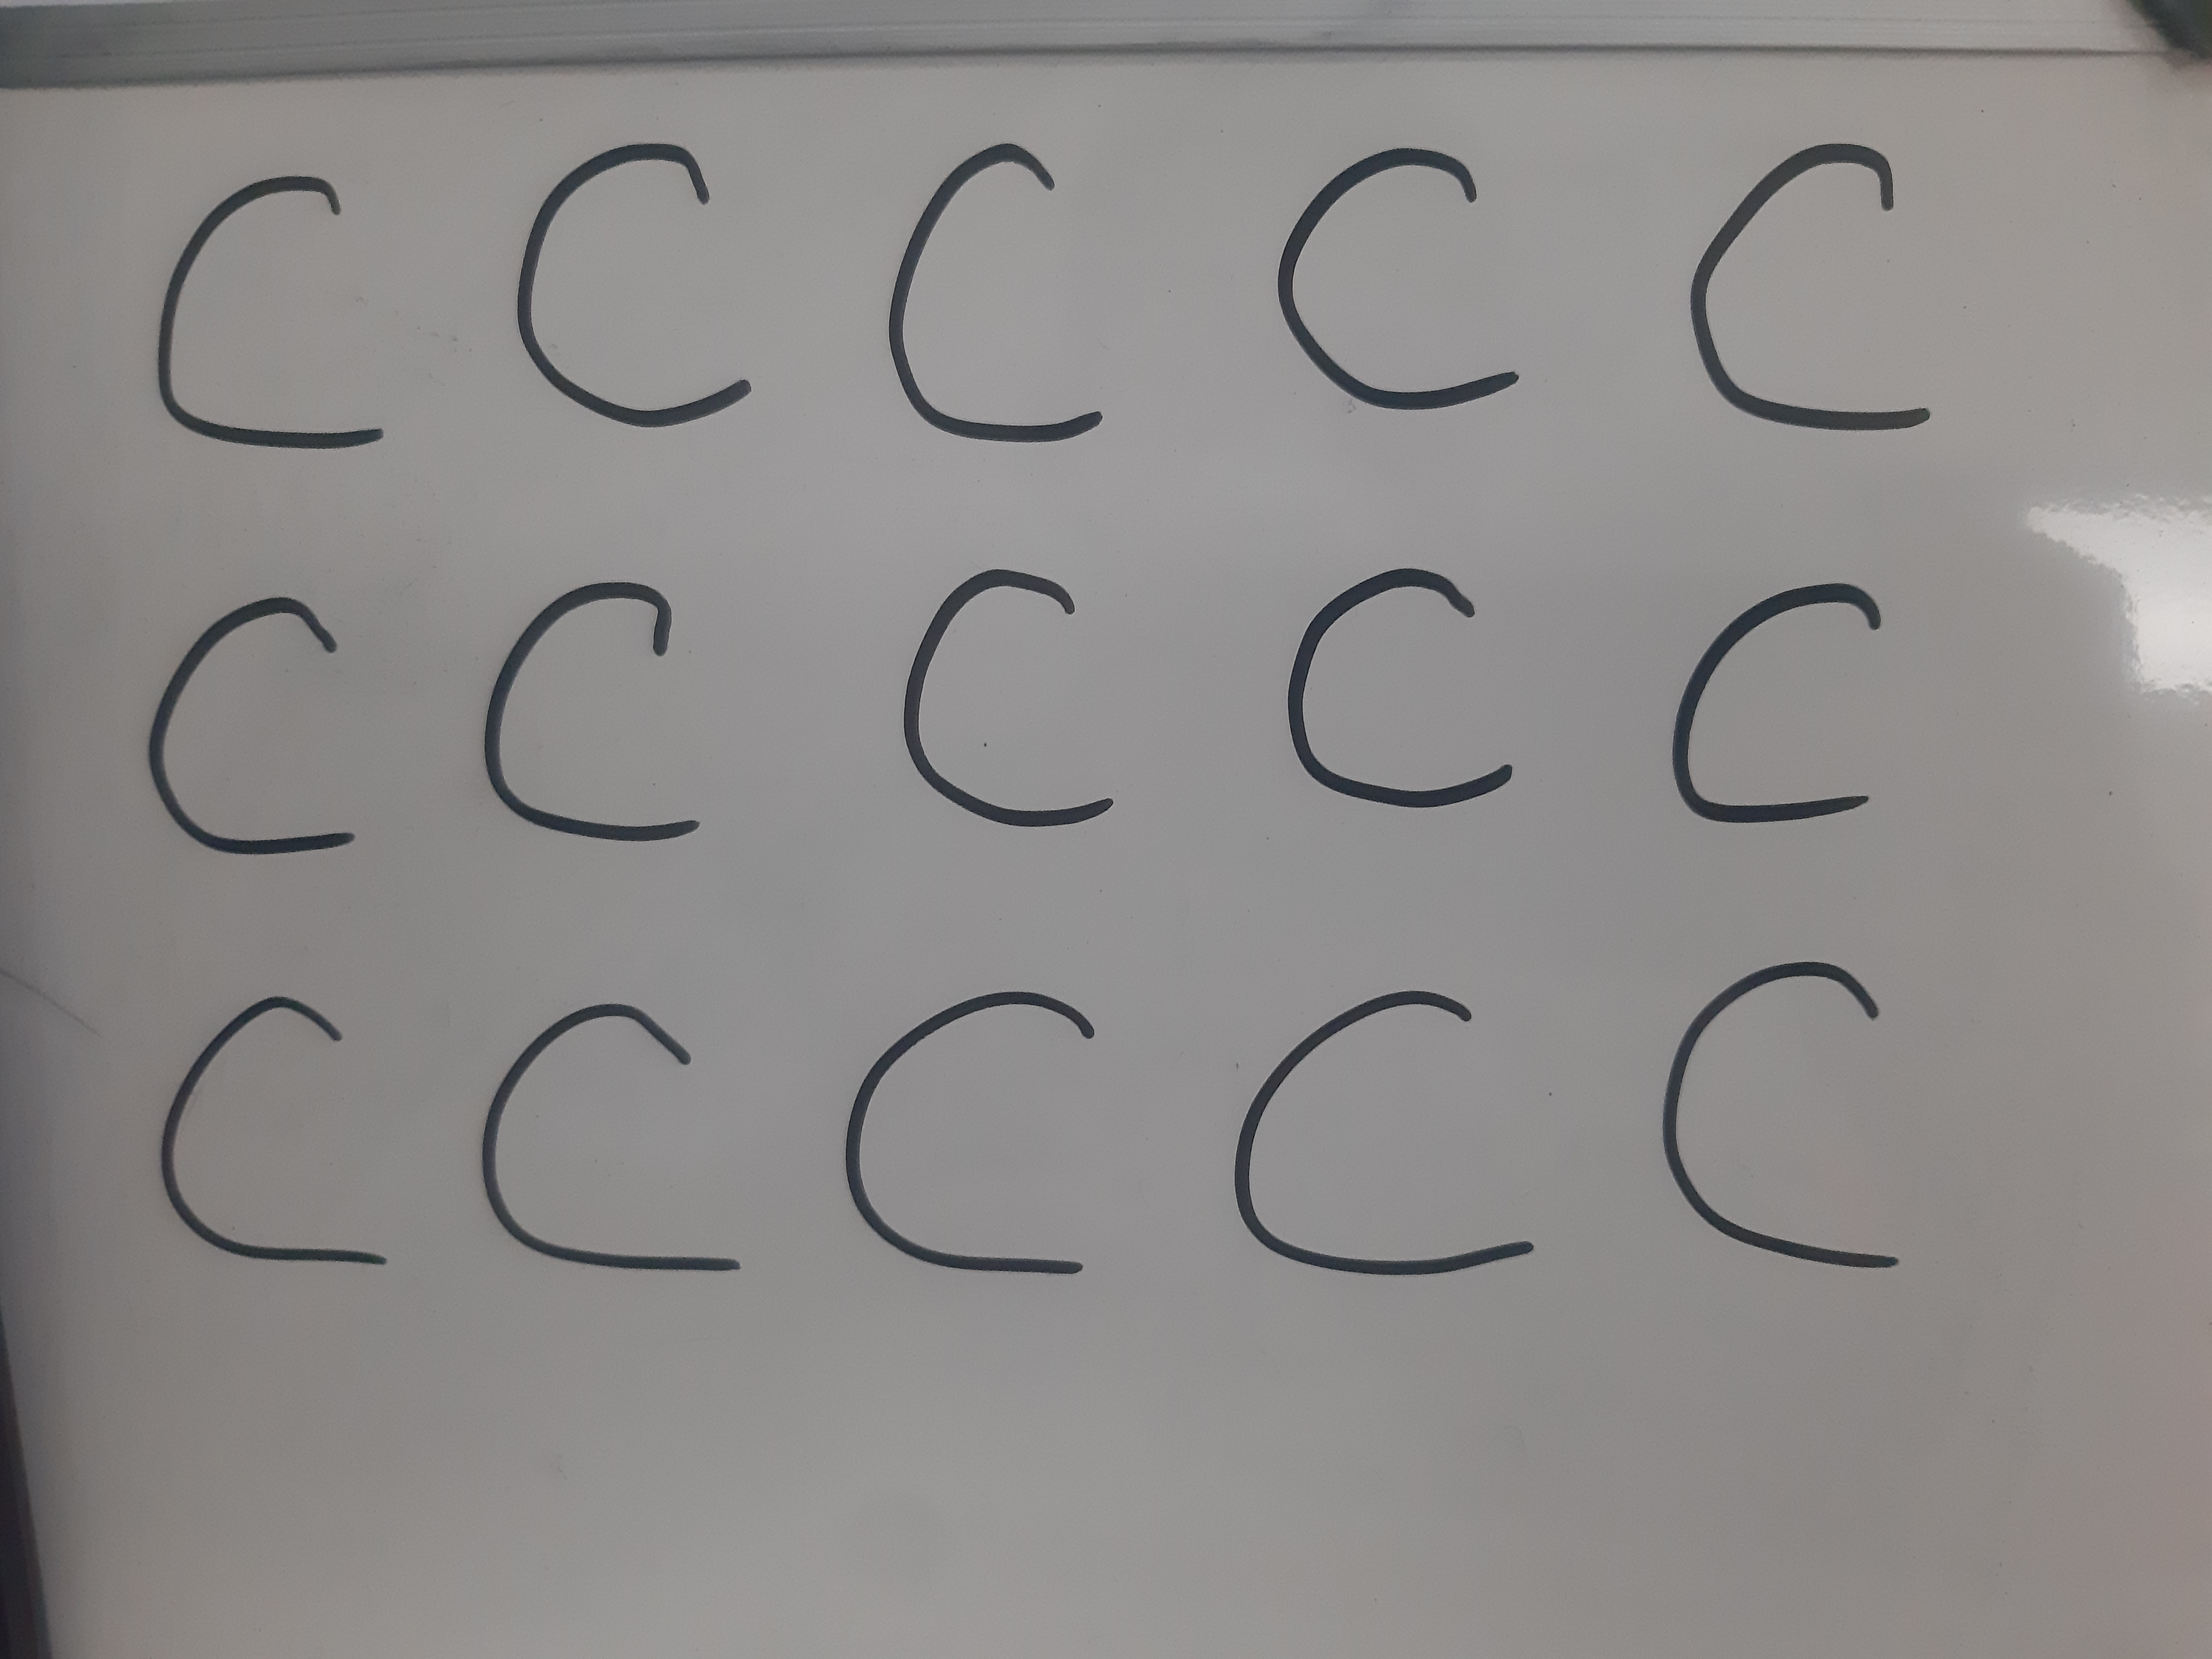
\includegraphics[scale=0.03]{gambar/c_dataset.jpg}
  \caption{Contoh Citra Tulisan Tangan pada Papan Tulis}
  \label{fig:contohcitratulisantangan}
\end{figure}

Adapun total persebaran gambar pada masing-masing kelas dapat dilihat pada tabel \ref{tb:citrapadatiapkelas} berikut. \par

\begin{table}[H]
  \begin{center}
    \begin{tabular}{|c|c|c|c|}
    \hline
    \textbf{Kelas} & \textbf{Jumlah Gambar} & \textbf{\textit{Train Sets}} & \textbf{\textit{Test Sets}} \\ \hline
    A                                    & 36                     & 29                  & 7                  \\ \hline
    B                                    & 36                     & 29                  & 7                  \\ \hline
    C                                    & 36                     & 29                  & 7                  \\ \hline
    D                                    & 36                     & 29                  & 7                  \\ \hline
    E                                    & 36                     & 29                  & 7                  \\ \hline
    F                                    & 36                     & 29                  & 7                  \\ \hline
    G                                    & 36                     & 29                  & 7                  \\ \hline
    H                                    & 36                     & 29                  & 7                  \\ \hline
    I                                    & 36                     & 29                  & 7                  \\ \hline
    J                                    & 36                     & 29                  & 7                  \\ \hline
    K                                    & 36                     & 29                  & 7                  \\ \hline
    L                                    & 36                     & 29                  & 7                  \\ \hline
    M                                    & 36                     & 29                  & 7                  \\ \hline
    N                                    & 36                     & 29                  & 7                  \\ \hline
    O                                    & 36                     & 29                  & 7                  \\ \hline
    P                                    & 36                     & 29                  & 7                  \\ \hline
    Q                                    & 36                     & 29                  & 7                  \\ \hline
    R                                    & 36                     & 29                  & 7                  \\ \hline
    S                                    & 36                     & 29                  & 7                  \\ \hline
    T                                    & 36                     & 29                  & 7                  \\ \hline
    U                                    & 36                     & 29                  & 7                  \\ \hline
    V                                    & 36                     & 29                  & 7                  \\ \hline
    W                                    & 36                     & 29                  & 7                  \\ \hline
    X                                    & 36                     & 29                  & 7                  \\ \hline
    Y                                    & 36                     & 29                  & 7                  \\ \hline
    Z                                    & 36                     & 29                  & 7                  \\ \hline
    \end{tabular}
  \end{center}
  
  \caption{Jumlah Citra Pada Tiap Kelas}
  \label{tb:citrapadatiapkelas}
  \end{table}

\subsubsection{Hasil Proses Pelabelan Dataset}
\label{subsubsec:hasilpelabelan}

Proses pelabelan dilakukan dengan memberikan \textit{bounding box} pada tiap citra yang telah dikumpulkan pada tahap sebelumnya. Proses pelabelan dapat dilihat pada gambar \ref{fig:labellingroboflow}. \par

\begin{figure}[H]
  \centering
  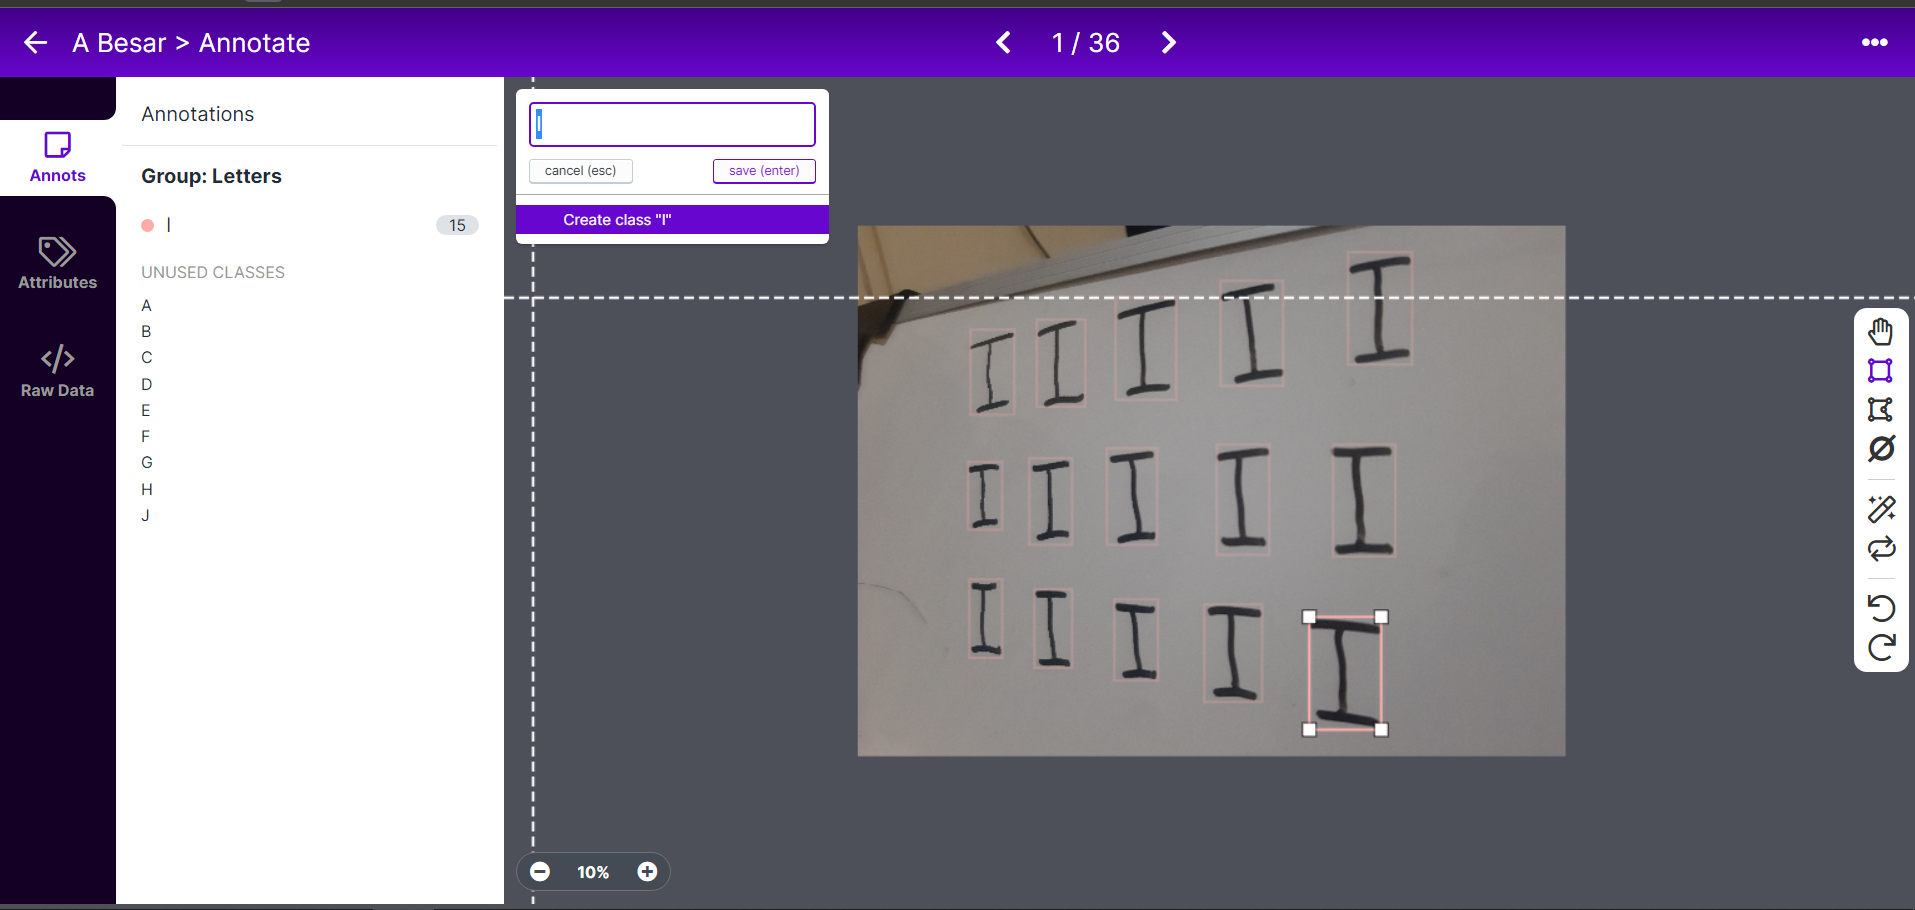
\includegraphics[scale=0.2]{gambar/labelling.png}
  \caption{Proses Pelabelan menggunakan Roboflow}
  \label{fig:labellingroboflow}
\end{figure}

Setelah dilakukan proses pelabelan, \textit{output} yang dihasilkan yaitu gambar yang memiliki \textit{bounding box}, dan apabila di-\textit{export} maka dataset hasil pelabelan terdiri dari 2 file yaitu file citra itu sendiri dan juga file txt yang berisi koordinat \textit{bounding box} yang ada pada suatu citra tersebut. Adapun total persebaran anotasi \textit{bounding box} pada masing-masing kelas dapat dilihat pada tabel \ref{tb:anotasitiapkelas} berikut. \par

\begin{table}[H]
  \begin{center}
    \begin{tabular}{|c|c|}
    \hline
    \textbf{Kelas} & \textbf{Jumlah Anotasi} \\ \hline
    A                                    & 540                     \\ \hline
    B                                    & 540                     \\ \hline
    C                                    & 540                     \\ \hline
    D                                    & 540                     \\ \hline
    E                                    & 540                     \\ \hline
    F                                    & 540                     \\ \hline
    G                                    & 540                     \\ \hline
    H                                    & 540                     \\ \hline
    I                                    & 540                     \\ \hline
    J                                    & 540                     \\ \hline
    K                                    & 540                     \\ \hline
    L                                    & 540                     \\ \hline
    M                                    & 540                     \\ \hline
    N                                    & 540                     \\ \hline
    O                                    & 540                     \\ \hline
    P                                    & 540                     \\ \hline
    Q                                    & 540                     \\ \hline
    R                                    & 540                     \\ \hline
    S                                    & 540                     \\ \hline
    T                                    & 540                     \\ \hline
    U                                    & 540                     \\ \hline
    V                                    & 540                     \\ \hline
    W                                    & 540                     \\ \hline
    X                                    & 540                     \\ \hline
    Y                                    & 540                     \\ \hline
    Z                                    & 540                     \\ \hline
    \end{tabular}
  \end{center}
  
  \caption{Jumlah Anotasi Pada Tiap Kelas}
  \label{tb:anotasitiapkelas}
  \end{table}

\subsubsection{Hasil Proses \textit{Image Pre-Processing}}
\label{subsubsec:hasilpreprocess}

Pada tahap \textit{pre-process}, citra yang telah diberi label selanjutnya diberikan sejumlah proses \textit{grayscalling} sehingga hasilnya seperti pada gambar \ref{fig:grayscallingdataset} dan \textit{bounding box rotation} sehingga hasilnya seperti pada gambar \ref*{fig:bbrotation}.

\begin{figure}[H]
  \centering
  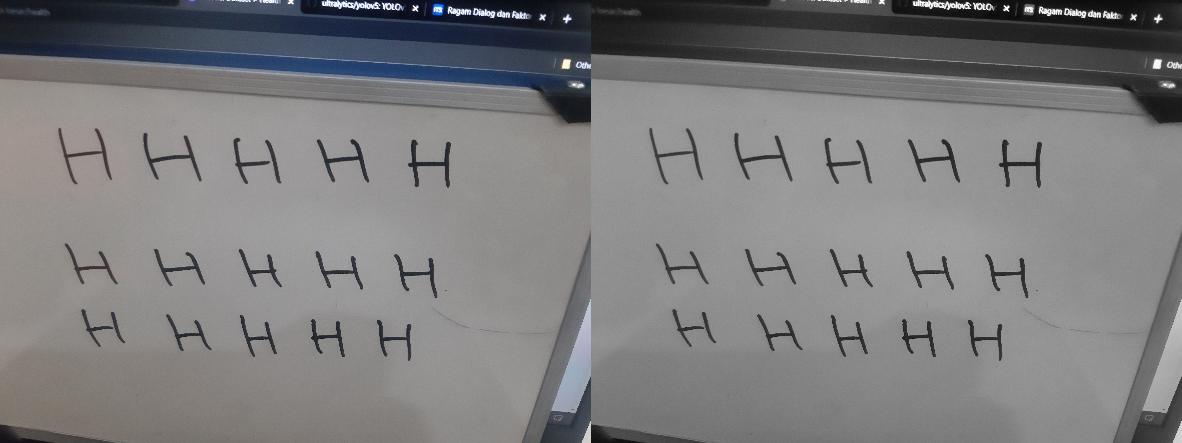
\includegraphics[scale=0.35]{gambar/grayscalling.png}
  \caption{Gambar Sebelum dan Setelah Proses \textit{Grayscalling}}
  \label{fig:grayscallingdataset}
\end{figure}

\begin{figure}[H]
  \centering
  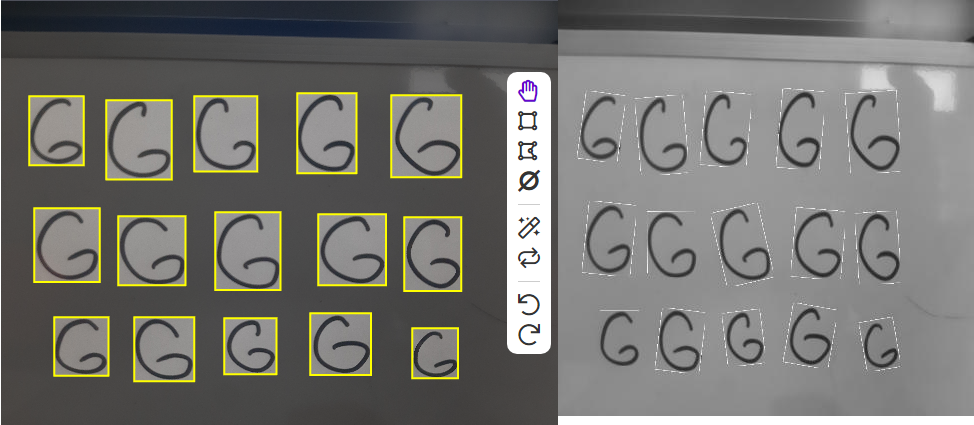
\includegraphics[scale=0.32]{gambar/bbrotation.png}
  \caption{Gambar Sebelum dan Setelah Proses \textit{Bounding Box Rotation}}
  \label{fig:bbrotation}
\end{figure}

\subsection{Hasil \textit{Training}}
\label{subsec:Hasiltraining}

Hasil \textit{training} data dilakukan setelah proses pengumpulan citra, proses pelabelan, dan pre-proses gambar selesai dilaksanakan. Hasil dari proses \textit{training} ini yaitu berupa model dan detil data angka pada tiap proses pengulangan  (epochs). Detil spesifikasi laptop yang digunakan dalam melakukan proses \textit{training} yaitu sesuai pada tabel \ref{tb:spesifikasilaptop}. Sedangkan detil parameter dan konfigurasi yang digunakan dapat dilihat pada tabel \ref*{tb:parametertrain} berikut. \par 

\begin{table}[H]
  \begin{center}
      \begin{tabular}{|l|c|}
      \hline
      \multicolumn{1}{|c|}{\textbf{Parameter}} & \textbf{Nilai} \\ \hline
      \textit{Weights}                         & YOLOv5s                 \\ \hline
      Epochs                                   & 30                      \\ \hline
      \textit{Batch-Size}                      & 16                      \\ \hline
      \textit{Image Size}                      & 416                     \\ \hline
      \end{tabular}
  \end{center}
  \caption{Detail Parameter yang Digunakan}
  \label{tb:parametertrain}
  \end{table}

Dari proses ini didapatkan hasil yaitu: \par
% grafik hasil training

Setelah didapatkan hasil model, dilakukan proses pengujian untuk menentukan apakah model tersebut sudah cukup akurat atau masih membutuhkan perbaikan. Pada proses pengujian didapatkan hasil bahwa model sudah dapat berfungsi seperti ditunjukkan pada gambar berikut. \par
% gambar pas detect model

\subsection{Hasil Pembuatan Model}
\label{subsec:hasilmembangunmodel}


\section{Skenario Pengujian}
\label{sec:skenariopengujian}

\section{Evaluasi Pengujian}
\label{sec:analisispengujian}
